% !TeX spellcheck = en_GB
\section{Part1: Advanced regression modelling}

Depending on the response variable (the value we'd like to model) a different model must be choosen.

\begin{tabular}{|l|l|}
	\hline 
	\textbf{Response} & \textbf{Model} \\ 
	\hline 
	Continuous (with condtant variance) & Multiple linear regression model \\ 
	\hline 
	Zero/one variate & Logistic regression model \\ 
	\hline 
	Counts & Loglinear model \\ 
	\hline 
	Continuous (with constant coefficient of variation) & Gamma regression model \\ 
	\hline 
	Censored survival times & Accelerated Failure Times Models \\
	& Proportional hazard model \\
	\hline 
\end{tabular} 

\subsection{Linear Regression (Recap)}

Form: $y \approx \beta_0 + \beta_1 x_i^{(1)} + ... + \beta_m x_i^{(m)}$\\
With $x_i^{1...m}$ being the \textbf{predictor variables} and $y$ the \textbf{response variable}. If $m=1$ the method is called \textbf{simple regression} otherwise \textbf{multiple regression}. While the \textbf{predictor variables} $x_i^{1...m}$ can be a non-linear combination of variables, the $\beta$s can only be multiplied (hence \textbf{linear regression}).

\subsubsection{Example R-Code}
\begin{lstlisting}
library(datasets) # the dataset mtcars is located in this package
str(mtcars) # Compactly displays the internal structure of the object
summary(mtcars) # returns a six number summary of each variable in the data frame

mtcars1 <- data.frame(lMPG=log(mtcars$mpg), wCyl=sqrt(mtcars$cyl),
					  lDisp=log(mtcars$disp), lHP=log(mtcars$hp),
					  drat=mtcars$drat, lWT=log(mtcars$wt),
					  qsec=mtcars$qsec, VS=mtcars$vs, AM=mtcars$am,
					  wGear=sqrt(mtcars$gear), wCarb=sqrt(mtcars$carb))

mtc1.lm1 <- lm(lMPG ~ lDisp + lHP + lWT + drat + qsec + wCarb + wCyl
               + wGear + VS + AM, data=mtcars1)
\end{lstlisting}

Inspecting the \lstinline{summary(mtc1.lm1)} output:
\begin{lstlisting}
Call:
lm(formula = lMPG ~ lDisp + lHP + lWT + drat + qsec + wCarb + 
wCyl + wGear + VS + AM, data = mtcars1)

Residuals:
Min       1Q   Median       3Q      Max 
-0.16637 -0.06968  0.01446  0.05770  0.20108 

Coefficients:
Estimate Std. Error t value Pr(>|t|)  
(Intercept)  3.733511   1.325541   2.817   0.0103 *
lDisp       -0.167383   0.179541  -0.932   0.3618  
lHP         -0.159416   0.134980  -1.181   0.2508  
lWT         -0.377992   0.250297  -1.510   0.1459  
drat         0.004172   0.074864   0.056   0.9561  
qsec         0.014235   0.033289   0.428   0.6733  
wCarb       -0.149562   0.115652  -1.293   0.2100  
wCyl         0.188301   0.217927   0.864   0.3973  
wGear        0.449734   0.264221   1.702   0.1035  
VS          -0.040222   0.088789  -0.453   0.6552  
AM          -0.054940   0.098564  -0.557   0.5831  
---
Signif. codes:  0 '***' 0.001 '**' 0.01 '*' 0.05 '.' 0.1 ' ' 1

Residual standard error: 0.1134 on 21 degrees of freedom
Multiple R-squared:  0.9018,	Adjusted R-squared:  0.8551 
F-statistic: 19.29 on 10 and 21 DF,  p-value: 2.097e-08
\end{lstlisting}

According to the F test for significance of regression, at least one of the explanatory variables is significant because its P-value of 3.649e-07 is smaller than 0.05. However, according to the marginal test none of the coefficients is significant on the 5\% level (except the intercept). This happens if the explanatory variables itself are (highly) correlated. To find a better model, a criterion must be chosen to find the optimal model.

\subsubsection{Akaike's information criterion}
A criterion to find better models:
\begin{equation*}
AIC = -2(maximized \: Log-Likelihood) + 2 \cdot \#estimates\: parameters
\end{equation*}
\begin{equation*}
AIC = n\cdot log(\frac{1}{n}\sum_{i=1}^{n} R_i^2) + 2p + constant
\end{equation*}
-> The criterion needs to be minimized

\paragraph{Use the R function \lstinline{step} to auto apply AIC}
\mbox{}
\begin{lstlisting}
mtc1.vs <- step(mtc1.lm1,
                scope=list(lower=~ 1,
                           upper=~ lDisp + lHP + drat + lWT + qsec
                                 + wCarb + fCyl + fVS + fAM + fGear))
\end{lstlisting}

While the variable \lstinline{mtc1.vs} now contains the model with the lowest AIC, a summary of the optimization process can be collected using \lstinline{mtc1.vs$anova}.

\paragraph{Compare two models using \lstinline{anova}}
ToDo %TODO

\subsubsection{Local Regression (LOESS)}
In comparison to linear model, where a \textbf{line} is fitted on the data, the LOESS regression can be used to fit a \textbf{curve}.

The concept of a LOESS regression is the following:

\begin{enumerate}
	\tightlist
	% See: https://www.youtube.com/watch?v=Vf7oJ6z2LCc
	\item For each point
	\begin{enumerate}
		\tightlist
		\item Set current point as \textbf{focal point}.
		\item Fit a straight line (\lstinline{family="gaussian"}) or a parabola (\lstinline{family="symetric"}) for the window. Inside the window, the distance of the point to the focal point determines the weight of each point.
		\item Set point at intercept with fitted line (\textbf{pre-fitted point})
	\end{enumerate}
	\item Calculate the difference for each point to the \textbf{pre-fitted point}
	\item For each pre-fitted point
	\begin{enumerate}
		\item Fit a line again using, but this time using the wights based on the distance to the \textbf{pre-fitted point}.
	\end{enumerate}
\end{enumerate}

\subsubsection{Residuals}

While the error term $E_i$ is unobservable it can be estimated by analysing the residuals:

\begin{equation*}
\vec{R} = \vec{Y} - \bm{X}\vec{\hat{\beta}} = \vec{Y} - \bm{H}\vec{Y} = (\bm{I}-\bm{H})\vec{Y}
\end{equation*}
\begin{equation*}
\bm{H} = \bm{X}(\bm{X}^T\bm{X})^{-1}\bm{X}^T
\end{equation*}

\paragraph{Scaled residuals}
\begin{equation*}
\breve{R_i} = \frac{R_i}{\sqrt{1-H_{ii}}}, i=1,...,n
\end{equation*}

\paragraph{Standardised residuals}
\begin{equation*}
\tilde{R_i} = \frac{R_i}{\sqrt{\hat{\sigma}^2(1-H_{ii}})}, i=1,...,n
\end{equation*}

\subsubsection{Diagnostic plots}
\begin{description}
	\tightlist
	\item[Tukey-Anscombe plot] Also called residual plot. Residuals against the fitted values: Is used to detect nonconstant expectation of the errors.
	\item[scale-lcation plot] The square-root of the absolute values of the standardized residuals against the fitted values: Is used to detect nonconstant variance of the errors.
	\item[normal Q-Q plot] Ordered standardized residuals against their expected values under normality: Is used to detect non normality of the errors.
	\item[Residuals against time and/or space variables] Is used to detect stochastic dependency in the errors.
	\item[sensitivity plot] Standardized residuals against leverage overlaid by Cook’s distance contours: Is used to detect too influential observation in the data.
\end{description}

\paragraph{Cook's distance}

\begin{equation*}
d_i = \frac{1}{p}\tilde{R_i}^2\frac{H_{ii}}{1-H_{ii}}
\end{equation*}

\textbf{Guideline:} Practical experience has shown that observations with a Cook’s distance $d_i$ larger than 1 can be considered as too influential.

\paragraph{Boostrap simulations}
Is an informal way to check stochastic fluctuation:
\begin{enumerate}
	\tightlist
	\item Generate observations $y_i^*$ according to the model using new random errors.\\
	$y_i^*=\hat{y_i}+\hat{\sigma}\cdot e_i^*$.
	\item Calculate the regression fit with the explanatory variables given in the data set and the newly generated response values $y_i^*$. Add the new lines to the plots.
	\item Repeat n times (n=19 for 5\% significance level).
\end{enumerate}

\subsubsection{Multicollinearity}
Is the term if some predictors are a linear combination of others.\\
Detect collinearity:
\begin{itemize}
	\tightlist
	\item Examination of the correlation matrix of the predictors will reveal large pairwise collinearities.
	\item The Variance Inflation Factor (VIF).\\
	\begin{lstlisting}
mtc3.lm0 <- lm(mpg ~ ., data=mtcars3)
vif(mtc3.lm0)
	\end{lstlisting}
	\textbf{Guideline:} If VIF is larger than 5 to 10 for any variable then multicollinearity is of a dangerous size and needs to be addressed.
\end{itemize}

\subsubsection{Categorical predictors}
If a predictor variable is categorical (e.g. a tool type) and has two levels, an indicator variable is set up:

\begin{equation*}
x_i = \begin{cases}
0 & if \; tool\; type\; A \\
1 & if\; tool\; type\; B
\end{cases}
\end{equation*}

In case of more than two levels, multiple indicator variables must be introduced:

\begin{tabular}{lll}
	$x_i^{2,2}$ & $x_i^{2,3}$  &  \\ 
	0 & 0 & for observation of type A \\ 
	1 & 0 & for observation of type B \\ 
	0 & 1 & for observation of type C \\ 
\end{tabular}

\subsubsection{Prediction error sum of squares (PRESS)}
In predictive modelling, the model are assessed often by the leave-one-out method. In this procedure, one observation is selected and the regression model is fitted to the remaining n-1 observations. With this we find the \textbf{prediction error for observation i}.
\begin{equation*}
r_{(i)}=y_i-\hat{y_(i)}
\end{equation*}
The \textbf{PRESS} is then defined by the sum of squares of the n prediction errors:
\begin{equation*}
PRSS = \sum_{i=1}^{n}r^2_{(i)} = \sum_{i=1}^{n}(y_i-\hat{y_{(i)}})^2
\end{equation*}

\subsubsection{Cross validation}
Cross validation is a model evaluation technique that tells how well the results will generalise to an independent dataset from the same population.\\
Basic idea (as example a 5-fold cross validation):
\begin{enumerate}
	\tightlist
	\item Split the data into n folds (for example chunks of 20\%)
	\item Use one fold for testing and the other for training
	\item Repeat step 2 n times until every fold is once used for testing
	\item Compute mean squared prediction error (MSPE)
	\begin{equation*}
		MSPE_{CV}=\frac{1}{n}\sum_{i=1}^{n}(\hat{y}_i^{Test} - y_i)^2
	\end{equation*}
\end{enumerate}

\subsubsection{Model building process}

\begin{enumerate}
	\tightlist
	\item Clarify the task (purpose? goal?); are there already model approaches?
	\item Data Screening and Processing
	\item Model fitting; preferably with robust methods
	\item Residual and sensitivity analysis; does this dataset help solve the task? -> Go back to 3, 2, 1 depending on the result
	\item Variable selection; treat collinearities if necessary -> Go back to 3 depending on the result
	\item Checking model adequacy
	\begin{itemize}
		\tightlist
		\item Residual and sensitivity analysis with selected model(s)
		\item Check plausibility; match model(s) with subject matter expertise
		\item Consider out-of-sample validation (i.e., validation with unused data), especially if the model is to be used for prediction.
	\end{itemize}
	-> Go back to 1, 2, 3, ... depending on the result
	\item Reporting: It is key to be honest and openly report all data manipulations and decisions that were made.
\end{enumerate}

\subsection{Advanced topics in linear regression modelling}

\subsubsection{Weighted least squares}

For the least squares regression to work, it is required to have an Error $\vec{E} \sim \mathcal{N}(\vec{0}, \sigma^2\bm{I})$ with $\bm{I}$ being the $n\times n$ identity matrix. In case of a \textbf{non-constant variance} called \textbf{heteroscedasticity} we need \textbf{weighted least squares} fitting. Therefore $\bm{I}$ is replaces with
\begin{equation*}
\bm{W}=diag[\frac{1}{w_1},\frac{1}{w_2}, ..., \frac{1}{w_n}] \neq \bm{I}
\end{equation*}

This allows us to give a weight for the samples we are more certain for the maximum likelihood calculation:

\begin{equation*}
\bm{X}^T\bm{W}\vec{R} = \vec{0}\;\; or \;\;
\bm{X}^T\bm{W}(\vec{Y}-\bm{X}\hat{\vec{\beta}}) = 0
\end{equation*}

\subsubsection{Robust fitting}
While real data is never exactly Gaussion distributed we need to find a model which is useful in many situations - hence for the majority of observations. The ordinary least squares (OLS) estimator cannot cope with this situation. A \textbf{robust} estimator is required.

\paragraph{The oldest, informal approach}

An easy common practise is to manually examine the data for obvious outliers and the manual removal of those. But this approach is problematic:
\begin{itemize}
	\tightlist
	\item Difficult or even impossible to identify outliers
	\item It is impossible to examine the relationship within the data without having a model in the first place
	\item The process of finding outliers is hard to formalize and therefore hard to automatize
	\item Inference based on applying a standard procedure to the cleaned data will be based on distribution theory which ignores the cleaning process and hence will be inapplicable and possibly misleading
\end{itemize}

\paragraph{Building a robust fitter}
By introducing weighted samples during the fitting process, samples with high residuals get applied a smaller wieght and therefore their influence is reduced.

\paragraph{M-estimator}
While the maximum likelihood estimator (OLS) tries to minimize the absolute residuals, the estimators belonging to the classes of M-estimators define a function $\rho$ which transforms the residuals (e.g. by clipping). Resulting in the following optimization function:
\begin{equation*}
\sum_{i=1}^{n}\psi(\tilde{r_i}) \cdot \vec{x_i} = \vec{0}
\end{equation*}
\begin{equation*}
\tilde{r_i} = \frac{Y_i-\vec{x_i}^T\vec{\hat{\beta_M}}}{\sigma}
\end{equation*}

The scale parameter $\sigma$ needs to be estimated. One possibility is to use the standard deviation, however this is extremely non-robust. It has been shown that a robust estimation is needed, called the MAV (=median of absolute value).
\begin{equation*}
	\sigma = s_{MAV} = \frac{median_i(|r_i|)}{0.6745}
\end{equation*}

\paragraph{MM-estimator}
\textbf{M}odified \textbf{M-estimator} improve the estimation of $\sigma$ since the M-estimator is not robust against leverage points. It uses the following procedure:
\begin{enumerate}
	\tightlist
	\item Find “good” initial values by optimising a slightly modified criterion (also called S-estimator)
	\item Apply a M-estimator but determine $\sigma$ from the estimation done in step 1.
\end{enumerate}

\subsubsection{Fitting smooth functions}
Another robust estimator is the \textbf{LOESS smoother} (\lstinline{loess.smooth}). It can either be fitted using an M-estimator (\lstinline{family="symmetric"}) oe by OLE (\lstinline{family="gaussian"}).

\paragraph{Cubic Spine Smoothing}
Is an alternative approach to local parametric regression for estimating a smooth function $f(\cdot)$ by a linear combination of some explicitly defined basis functions $h_m(\cdot)$. The number M controls the smoothness and the complexity of $f(\cdot)$.

\begin{equation*}
f(x) = \sum_{m=1}^{M}\gamma_m h_m(x)
\end{equation*}

This is highly subjected to overfitting for large M. Therefore the minimization function must penalized in case of high complexity. This can be achieved by introducing a function measuring the curvature.
\begin{equation*}
\sum_{i=1}^{n}(y_i-f(x_i))^2 + \lambda \int_{-\infty}^{\infty}f''(u) du
\end{equation*}

When analysing the above function it can be seen that $\lambda$ can also be fitted by doing a cross validation (e.g. leave-one-out) that it minimizes the expected squared prediction error.

\paragraph{Additive regression model and backfitting algorithm}
The cubic spine smoothing can be generalised to \textbf{(generalised) additive models}:
\begin{equation*}
Y_i = \beta_0 + f_1(x_i^{(1)}) + ... + f_m(x_i^{(m)}) + E_i
\end{equation*}

To estimate the flexible components for each predictor the backfitting algorithm is used:
\begin{enumerate}
	\tightlist
	\item Initialize $\hat{\beta_0} = \bar{y}$ and $\hat{f_k}(\cdot)=0$ for all $k=1, ..., m$ predictor variables
	\item Repeat for all $k=1, ..., m$ until convergence:
	\begin{enumerate}
		\tightlist
		\item Compute the partial residual $\tilde{y_i}^{(k)} = y_i - \hat{\beta_0}-\sum_{j=1, j\neq k}^{m} \hat{f_j}(x_i^{(j)})$
		\item Solve the 1-d smoothing problem using the data $(x_i^{(k)}, \tilde{y_i}^{(k)}) \rightarrow \hat{f_k}(\cdot)$
		\item Center the estimated function to $\hat{f_k}(\cdot) \leftarrow \hat{f_k}(\cdot) - \frac{1}{n} \sum_{i=1}^{n} \hat{f_k}(x_i^{(k)})$
	\end{enumerate}
\end{enumerate}

\subsection{Binary response}

\subsubsection{Sunflower-Plot and proportion plot}

The problem when plotting binary response variables is, that there are many measurements ``on the same point''. One way to overcome this problem when plotting binary response variable is to introduce a sunflower symbol for plotting. For every overlapping measurement, a new leaf is added to the sunflower.
\begin{figure}[H]
	\centering
	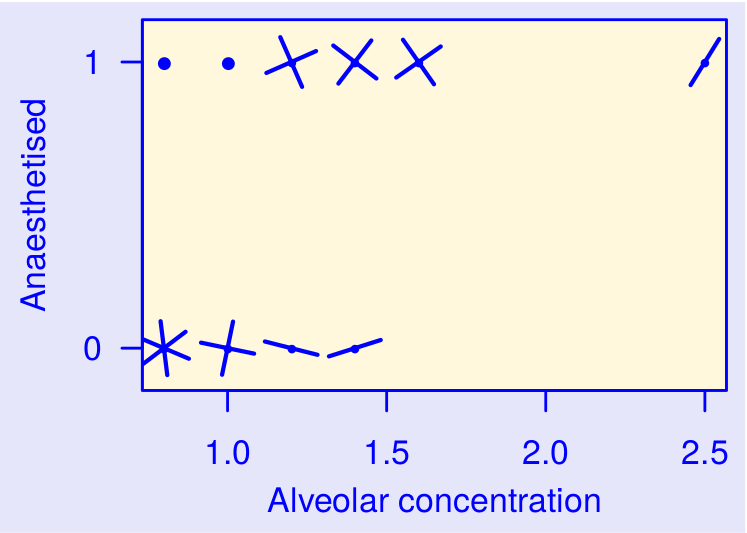
\includegraphics[width=0.3\textwidth]{images/sunflower.png}
	\caption{Example sunflower plot}
\end{figure}

Another way of visualizing binary data is by calculating the proportion of ``ones'' for each corresponding input value $x$. The aggregated data $\tilde{Y_k}$ can then be plotted again using the sunflower plot.

\subsubsection{Logistic regression}

The problem when using linear regression is, that the prediction is not bounded. While the aggregated $\tilde{Y_k}$ is always within the interval $[0, 1]$ the predicted value can be outside of this range.

\mbox{}\\
Such a logistic regression must have the following properties:
\begin{enumerate}
	\tightlist
	\item The response Y is binary with possible values 0 and 1.\\
	In other words: $Y \sim Bernoulli(\pi=unknown)$
	\item $E(Y) = \pi$
	\item $\pi(x_k) = G(\beta_0 + \beta_1 \cdot x_k)$ or $G^{-1}(\pi(x_k)) = \beta_0 + \beta_1 \cdot x_k$\\
	With $x_k$ being the predictor variables and $G$ a distribution function.
	\item This results in a latent variable $Z =\eta(x_k) = \beta_0 + \beta_1 \cdot x_k$. The response $Y$ maps $\eta$ to 1 if $Z > c$ or vice versa.
	\item According to point 3: $\eta = G^{-1}(\pi)$. With $G^{-1}$ as \textbf{link function}.
\end{enumerate}

\paragraph{Popular choices for the distribution ($G()$) and link function ($G^{-1}()$)}\mbox{}\\
\begin{tabular}{ccl}
	\hline 
	$G(\eta)$ & $G^{-1}(\pi)$ & Name \\ 
	\hline 
	$\exp(\eta)/(1+\exp(\eta))$& $log(\pi/(1-\pi))$  & logit model; logistic regression (generally preferred) \\ 
	$\phi(\eta)$ & $\phi^{-1}(\eta)$ & probit model \\
	$1-exp(-exp(\eta))$ & $log(-log(1-\pi))$ & complementary log-log model \\
	\hline 
\end{tabular}

\paragraph{Odds}
Instead of focusing on the probability of occurrence of an event we turn our attention to the ‘odds’ for success versus failure:
\begin{equation*}
odds = \frac{P(Y_i=1)}{P(Y_i=0)} = \frac{P(Y_i=1)}{1 - P(Y_i=1)} = \frac{\pi}{1-\pi}
\end{equation*}

Since the range of odds is between 0 and infinity, the log-odds (logarithmic odds) are often preferred:
\begin{equation*}
log(odds) = log(\frac{\pi}{1-\pi}) = \eta = \beta_0 + \sum_{j=1}^{m} \beta_j x^{(j)}
\end{equation*}

\paragraph{Empirical logits}

Because the logit model is not defined for $G^{-1}(0)$ and $G^{-1}(1)$ (Latent variable $Z = g(Y)$) the empirical logits are often used:
\begin{equation*}
Z_k = log(\frac{Y_k + 0.5}{m_k-Y_k+0.5})
\end{equation*}

\subsubsection{Maximum Likelihood Estimator (MLE)}

While the previously introduced estimators (e.g. least squares estimator) is good for fitting continuous (Gaussian like) data, it is not suitable for binary response variables where the response is either 0 or 1. In comparison th MLE is better suited for fitting non Gaussian like data because it can work with any distribution since it fits the parameter of the distribution.

\subsection{Generalised linear model}

The components introduced for logistic regression can be summarized and generalized even further if the following properties are given:

\begin{itemize}
	\tightlist
	\item A set of explanatory variables ($x^{(1)}, x^{(2)}, ..., x^{(m)}$)
	\item A response variable $Y$ with expectation $E(Y)=\mu$
	\item A link function $G^{-1} = g$ such that $g(\mu) = \vec{x}^T \vec{\beta}$
	\item A distribution for the variability in $Y$
\end{itemize}

These conditions are met if the probability function $f$ of $Y$ can be written as
\begin{equation*}
f(y_i, \mu_i, \phi) = exp(\frac{y_i b(\mu_i)-c(\mu_i)}{\phi}w_i+d(y_i, \phi, w_i))
\end{equation*}
With:
\begin{description}
	\tightlist
	\item[$b()$ and $c()$] Determine the specific distribution
	\item[$d()$] Normalizes the function to a total of 1
	\item[$\phi$] Dispersion parameter
	\item[$w_i$] Known number but may vary from observation to observation.	It has the meaning of a weight.
\end{description}

This results in the following parameters for common distributions:

\begin{tabular}{l||rr|rrcc}
	\hline 
	Distribution & $E(Y) = \mu$ & $var(Y)$ & $b(\mu)$ & $V(\mu)$ & $\phi$ & w \\
	\hline
	$Gaussion(\mu, \sigma^2)$ & $\mu$ & $\sigma^2$ & $\mu$ & 1 & $\sigma^2$ & 1\\
	$Binomial(m, \pi)$ & $m\cdot\pi$ & $\frac{1}{m}\pi(1-\pi)$ & $log(\frac{\mu}{1-\mu})$ & $\mu(1-\mu)$ & 1 & m\\
	$Poisson(\lambda)$ & $\lambda$ & $\lambda$ & $log(\mu)$ & $\mu$ & 1 & 1\\
	$Gamma(\alpha, \beta)$ & $\frac{\alpha}{\beta}$ & $\frac{\alpha}{\beta^2}$ & $-\frac{1}{\mu}$ & $\mu^2$ & $\frac{1}{\alpha}$ & 1\\
	\hline
\end{tabular}

\paragraph{Link function}
The corresponding inverse link function $G() = g^{-1}()$ should map the values of the linear predictor $\eta = \vec{x}^T \vec{\beta}$ to the support of the expected value of $Y$.\\
Obvious link functions:
\begin{description}
	\item[Identity] $g(\mu) = \mu$ if $Y$ is not subject to any restrictions on $\mathbb{R}$
	\item[Log] $g(\mu) = log(\mu)$ if $Y$ must be a positive real number
	\item[Logit] $g(\mu) = logit(\mu)=log(\mu/(1-\mu)$ if $Y$ must be between 0 and 1 (e.g. logistic regression)
\end{description}

\paragraph{Canonical link}
For every distribution a so called canonical link function (clf) exists which transforms $\eta$ to the defined distribution.

\paragraph{Support in R}
\lstinline{glm(..., family=poisson(link=identity))} a GLM can be fitted using different link functions. The default function is the canonical link function.

\begin{tabular}{c|cccccc}
	& binomial & gaussian & Gamma & inverse.gaussian & poisson & quasi \\
	\hline 
	logit & D & & & & & x \\
	probit & x & & & & & x \\
	cauchit & x & & & & &  \\
	clolog & x & & & & & x \\
	identity & & D & x & & x & x \\
	inverse & & & D & & & x \\
	log & x & & x & & D & x \\
	$1/\mu^2$ & & & & D & & x \\
	sqrt & & & & & x & x \\
\end{tabular}

\subsubsection{Fitting a GLM}

Like a logistic model, a GLM is also fitted using a maximum likelihood estimator (MLE). For a robust fitting the \textbf{IRLS (Iteratively reweighted least squares) algorithm} can be used. It is basically a weighted MLE estimator to lower the influence of outliers.

\subsection{Model simplification and variable selection}

The F-Score cannot be used for generalized linear models, since we cannot formulate an appropriate test statistic.

\subsubsection{Residual deviance}

The residual deviance is defined as:
\begin{equation*}
RD = 2\cdot (log-likelohood(M_S) - log-likelihood(M_P)) \sim \chi^2(df(M_S) - df(M_P))
\end{equation*}

With $M_S$ being the more saturated model and $M_P$ the proposed model. The $df()$ operator gets the degrees of freedom. The full saturated model or saturated model is a model which has the same amount of parameters as observations.

\paragraph{Deviance Test}
The deviance test is the F test counterpart to check if the proposed model is significantly better than saturated model. For this the p-value of $RD$ following a  $\chi^2(df(M_S) - df(M_P))$ distribution is calculated.

\begin{lstlisting}
DaR.glm <- glm(RDR ~ lPOP + lAR + lHR + lVH + lF+ IND, family=poisson,
data=DaR)
DaR.glm2 <- glm(RDR ~ lAR + lHR + lVH + IND, family=poisson, data=DaR)
anova(DaR.glm, DaR.glm2, test="Chisq")
\end{lstlisting}

\paragraph{Null deviance}
The null deviance can be used as an analogy for the F-test. Since the null deviance is the deviance of the null model (using the intercept only), a deviance test can be used to check if the found model is significantly better than the null model.

\begin{lstlisting}
MAC1.glm1 <- glm(cbind(Y, m-Y) ~ ac, family=binomial, MAC1)
summary(MAC1.glm1)
...showing just the deviance lines ...
Null Deviance: 15.4334 on 5 degrees of freedom
Residual Deviance: 1.7321 on 4 degrees of freedom

1- pchisq(15.4334 - 1.7321, df=1)
\end{lstlisting}

\paragraph{Variable selection}
AIC and stepwise model selection can also be used for GLMs.

\subsubsection{Confidence intervals}

There are two approaches for finding the confidence interval of GLMs, the \textbf{delta method} and \textbf{finding the confidence interval for $\eta$}.

\paragraph{Delta method}
Using the delta method, the confidence intervals are found using a Taylor expansion of $G(\vec{x_0^T}\vec{\hat{\beta}})$ at $\vec{x_0^T}\vec{\beta}$:

\begin{equation*}
G(\vec{x_0^T}\vec{\hat{\beta}}) \approx G(\vec{x_0^T}\vec{\beta}) + G^{'}(\vec{x_0^T}\vec{\beta}) (\vec{x_0^T}\vec{\hat{\beta}} - \vec{x_0^T}\vec{\beta})
\end{equation*}

Resulting in an approximately Gaussian distributed $G(\vec{x_0^T}\vec{\hat{\beta}})$:
\begin{equation*}
G(\vec{x_0^T}\vec{\hat{\beta}}) \sim \mathcal{N}\left (G(\vec{x_0^T}\vec{\beta}),\; G^{'}(\vec{x_0^T}\vec{\beta})^2 \vec{x_0}^T cov(\vec{\hat{\beta}})\vec{x_0}\right)
\end{equation*}

Therefore:
\begin{equation*}
G(\vec{x_0^T}\vec{\hat{\beta}}) \pm x_i = \begin{cases}
q^\mathcal{N}_{1-\alpha/2}se(\hat{\mu_0};\phi=1) & if\; \phi = 1 \\
q^{t_{n-p}}_{1-\alpha/2}se(\hat{\mu_0};\hat {\phi}) & if\: \phi\: has\: to\: be\: estimated
\end{cases}
\end{equation*}
with:
\begin{equation*}
se(\hat{\mu_0};\phi) = \sqrt{\phi \left(h^{'}(\vec{x_0^T}\vec{\hat{\beta}})\right)^2 \vec{x_0}^T\bm{(X^TWX)^{-1}}\vec{x_0}}
\end{equation*}

\paragraph{Deviance based method}
The approximation of the delta method (a.k.a \textbf{Wald test statistic}) is not good enough in all situations.

\begin{equation*}
T_D = \frac{D(\vec{y};\vec{\hat{\beta^{*k}}})-D(\vec{y};\vec{\hat{\beta}})}{\hat{\phi}} \leq q^{\chi^2_1}_{1-\alpha}
\end{equation*}

With $\beta^{*k}$ as the limit of the $\alpha$ confidence interval.

\subsection{Diagnostics and model improvement}

\subsubsection{Estimation of the dispersion parameter $\phi$}

Depending on the data structure which need to be fit, a different estimator is used:

\paragraph{Gaussian model}
\begin{equation*}
\phi = \sigma^2 = MSE = \frac{1}{n-p}\sum_{i=1}^{n}(Y_i - \hat{\mu_i})
\end{equation*}

\paragraph{Gamma model}
\begin{equation*}
CV = \frac{1}{n-p}\sum_{i=1}^{n}\left(\frac{Y_i-\hat{\mu_i}}{\hat{\mu_i}}\right)^2
\end{equation*}

\paragraph{Binomial, Poisson and exponential models}
With these models $\phi = 1$. Therefore, no estimation is required.

\paragraph{Overdispersion}

If $D \sim \chi^2_{n-p}$ is very unlikely an overdispersion happens. The most common case is the wrong structural form for the model. Other cases are:
\begin{itemize}
	\tightlist
	\item The presence of a few outliers
	\item Many points are identified as outliers
\end{itemize}

To check for overdispersion check if your residual deviance is $\chi^2_{df}$ distributed:
\begin{lstlisting}
1-pchisq(<residual-deviance>, <df-residual-deviance>)
\end{lstlisting}

\subsubsection{Diagnostics -  Model adequacy checking}
For GLMs there is no such thing a well-defined definition of residuals. The matrix $\bm{H}$ of a GLM fit is:
\begin{equation*}
\bm{H}=\bm{W}^{1/2}\bm{X}(\bm{X}^T\bm{W}\bm{X})^{-1}\bm{X}^T\bm{W}^{1/2}
\end{equation*}

\paragraph{Response residuals} The simplest method of defining a residual. Generally, note that $R_i$ will not be Gaussian distributed. 
\begin{equation*}
R_i = Y_i - \hat{\mu_i}
\end{equation*}

\paragraph{Pearson residuals}
Often used. However, still not Gaussian distributed.
\begin{equation*}
R_i^{(P)} = R_i \cdot w_i/\sqrt{(V(\hat{\mu_i}))}
\end{equation*}

With $V(\cdot)$ as the variance function.

\paragraph{Working residuals}
These residuals mimic the residuals from classic linear models. However, they cannot be used to estimate the scale parameter $\phi = \sigma^2$ using the residual sum of squares. 
\begin{equation*}
R_i^{(W)} = R_i\cdot g'(\hat{\mu_i})
\end{equation*}

\paragraph{Deviance residuals}
A definition of residuals to be used to estimate the scale paramater are the deviance residuals.
\begin{gather*}
R_i^{(D)} = sign(y_i - \hat{\mu_i})\sqrt{d_i} \\
var\left(R_i^{(D)}\right)\approx \phi(1-H_{ii})
\end{gather*}

\subsubsection{Residual analysis}
The residual analysis of GLMs differs from the one known in OLS slightly.

\paragraph{Tukey-Anscombe plot}
(Also called residual plot) In comparison to linear models, the Tukey-Anscombe plot plots the deviance residuals $R_i^{(D)}$ against the fitted linear predictor $\hat{\eta_i}$. When having a discrete response, caution is required, because the discreteness introduces distortion.\\
It can be used to examine if the deviance does ``not depend on the linear predictor''. In case the plot is not around zero all the time, either dangerously influential outliers are within the data or the model choice is bad.\\
Implies that the assumption of a constant expectation of the error holds.

\paragraph{Scale-Location Plot}
In order to investigate the dependence of the variance on the fitted values, the scale-location plot is used. It plots the square-root of the absolute values of the standardized deviance residuals against the fitted linear predictor.\\
In case there is nor flat line, the plot suggests, that there is a non-constant variability in the residuals. Hence, not all variance is captured by the model.

\paragraph{Normal Q-Q Plot}
Can only be used to interpret the response of non-binary responses and must be handled with care. In many cases, the residuals are not normally distributed or show great values even though the model does not fit the data.\\
However, the plot is useful to examine overdispersion. It helps to determine if overdispersion happens due to a few outliers (non-linearity due to large residuals) or due to the assumed distribution being inappropriate (non-linearity due to large and small residuals).

\paragraph{Residual vs leverage plot}
We need to identify the leverage points and influential observations in addition to outliers. The cook's distance can also be used for GLMs:
\begin{equation*}
d_i = \frac{1}{p}\frac{R_i^2}{\hat{\phi}\cdot V(\hat{\mu_i})(1-H_{ii})}\frac{H_{ii}}{1-H_{ii}}
\end{equation*}
Observation with $d_i \geq 1$ are considered dangerously influential.

Rule of thumb for high leverage:
\begin{equation*}
	L_{crit} = 2\cdot \frac{p}{n}
\end{equation*}
With $n$ as the number of samples and $p$ the rank of the hat matrix $\bm{H}$ (which is equal to the number of $\beta$s).

\subsubsection{Generalised Additive Models (GAM)}
These models extend the GLMs by replacing some or all linear terms of $\eta$ with appropriate smooth functions:
\begin{equation*}
\eta_i = \beta_0+\sum_{k=1}^{m}x_i^{(k)}\beta_k \; \rightarrow \; \eta_i = \sum_{k=1}^{m}f_k\left(x_i^{(k)}\right)
\end{equation*}
The GAMs are mainly used to fine appropriate transformations of explanatory variables.

\subsection{Some extensions of GLM}

\subsubsection{Categorical responses}
In case the response is categorical with more than two levels it is an extension of the binomial regression model. Generally it is distinguished by:
\begin{description}
	\tightlist
	\item[Nominal data] where there is no natural order to the response	categories.
	\item[Ordinal data] where there is an order in the data.
\end{description}

\paragraph{Contingency table}
A contingency table is a type of table in a matrix format that displays the (multivariate) frequency distribution of categorical variables. Example:
\begin{lstlisting}
table(USes96$fAge, USes96$Party)
           Democrat Independent Republican
(0,25]         33          15         18
(25,35]        76          54         73
(35,45]        89          59         85
(45,55]        68          48         52
(55,65]        49          24         40
(65,75]        41          24         34
(75,100]       24          15         23
\end{lstlisting}

\paragraph{Mosaic plot}
One way to visualize contingency tables is by using Mosaic plots. An example of those plots is shown bellow:
\begin{figure}[H]
	\centering
	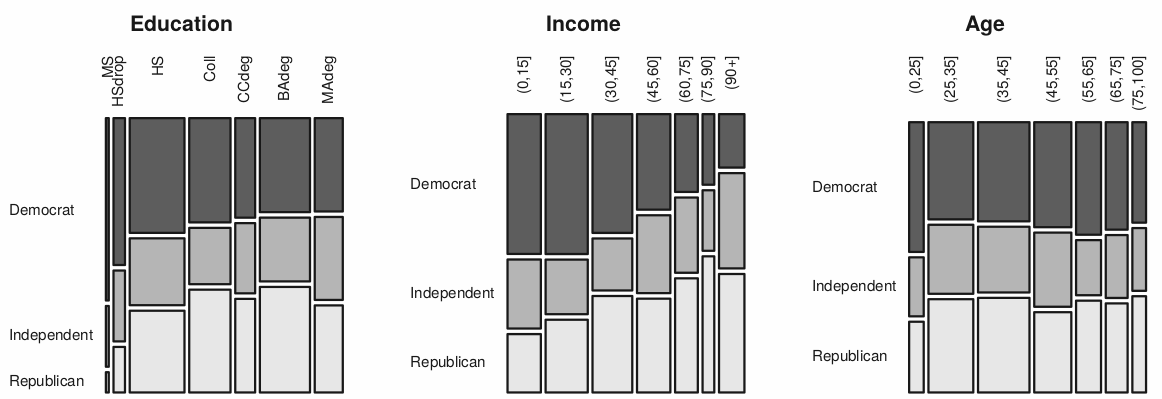
\includegraphics[width=.8\textwidth]{images/example-mosaic.png}
	\caption{Example visualization using a mosaic plot}
\end{figure}

\subsubsection{Multinomial logit model}
Let $Y_l$ be a random variable coding response categories with values $1, 2, ..., L$. The probability for sample $i$ to be in category $l$ is known as $\pi_{il}$. The number of observation in category $l$ is known as $y_{il}$ and $n_i$ the number of individuals in observation $i$.
\begin{equation*}
n_i = \sum_{l=1}^{L}y_{il}
\end{equation*}

R-Code:
\begin{lstlisting}
library(nnet)
multinom(Party ~ fAge + income + educ, data=USes96)

# weights:  60 (38 variable)
initial  value 1037.090001 
iter  10 value 979.148422
iter  20 value 976.235668
iter  30 value 976.101052
iter  40 value 976.098777
iter  40 value 976.098774
iter  40 value 976.098772
final  value 976.098772 
converged
Call:
multinom(formula = Party ~ fAge + income + educ, data = USes96)

...

Residual Deviance: 1952.198 
AIC: 2028.198 
\end{lstlisting}

\paragraph{Inference}
To check if the $k^{th}$ explanatory variable has a significant impact it is not possible to perform an individual hypothesis test. Unfortunately, \lstinline{anova()} is not able to do this calculation, we have to do them manually:
\begin{lstlisting}
mn1 <- multinom(Party ~ fAge + income + educ, data=USes96)
mn2 <- multinom(Party ~ fAge + income, data=USes96)

# Difference of deviances
h1 <- deviance(mn2) - deviance(mn1)
# Difference of df
h2 <- abs(mn1$edf - mn2$edf)
# p-value calculation
pchisq(h1, h2, lower=FALSE)
\end{lstlisting}

\paragraph{Predict}
To show the probability of samples belonging to a certain class use:
\begin{lstlisting}
predict(USes96.mn2, type="probs")
\end{lstlisting}
In case only the class needs to be known \lstinline{type="class"} can be used.

\subsubsection{Ordinal multinomial responses}
Multinomial responses are still categorical, but with a natural ordering among the categories.\\
Example Mental Impairment: The goal was to relate mental impairment to socio-economic status and the frequency of potentially traumatic events in a persons’ life. The response variable has the following values: none, mild, moderate and impaired.

\mbox{}\\
When using ordinal multinomial response, it is possible to work with cumulative probabilities:
\begin{equation*}
\gamma_{il} = P(Y_i\leq l)
\end{equation*}

This approach makes it possible to model only (L-1) probabilities.

R-Code:
\begin{lstlisting}
TODO: Code from slides does not work
\end{lstlisting}

\paragraph{Inference}
For ordinal multinomial responses \lstinline{anova} can be used for comparison:

\paragraph{Prediction}
Identical properties as the multinomial logit model.
